\documentclass[10pt]{beamer}
\mode<presentation>
\usepackage{beamerthemesplit}
\usepackage{graphicx}
\usepackage{booktabs}
\usepackage{amsmath}
\usepackage{textpos}
% \usepackage[linesnumbered,ruled,vlined]{algorithm2e}
\usepackage{pgfplots}
\usepackage{tikz}
\usepackage{hyperref}
% \usepackage{caption}
\usepackage{listings}
\usepackage{algorithm}
% \usepackage{algpseudocode}
\usepackage{algorithmic}
% \usepackage[backend=biber, style=numeric]{biblatex}


% import citation package
\usepackage{biblatex}
\addbibresource{presentation.bib}
\AtBeginBibliography{\small}

\usetikzlibrary{shapes.geometric, arrows}
\usetikzlibrary {datavisualization} 
\pgfplotsset{compat=1.18, width = 7cm}
\usetikzlibrary{patterns}
\usetheme{Ilmenau} % AnnArbor, Ilmenau, Darmstadt, Dresden, CambridgeUS, Frankfurt, Singapore
\newtheorem{dn}{Định nghĩa}[section]
\newtheorem{dl}{Định lý}[section]
\newtheorem{tc}{Tính chất}[section]
\newtheorem{hq}{Hệ quả}[section]
\newtheorem{bd}{Bổ đề}[section]
\newtheorem{md}{Mệnh đề}[section]
\newtheorem{vd}{Ví dụ}[section]
\newtheorem{nx}{Nhận xét}[section]
\newtheorem{cy}{Chú ý}[section]
\newcommand{\dom}{\text{{\rm dom}}}
\newcommand{\epi}{\text{{\rm epi}}}
\newcommand{\Min}{\text{{\rm Min}}}
\setbeamertemplate{theorems}[numbered]
\setbeamertemplate{definitions}[numbered]
\setbeamertemplate{footline}[frame number]
\usepackage{algorithm}
\usepackage{color}
\usepackage{algorithmic}
\usepackage{footmisc}
\usepackage{indentfirst} 
\usepackage{comment}
\AtBeginEnvironment{proof}{%
  \setbeamercolor{block title}{use=example text,fg=white,bg=example text.fg!75!black}
  \setbeamercolor{block body}{parent=normal text,use=block title example,bg=block title example.bg!10!bg}
}
\renewcommand{\thefootnote}{\arabic{footnote}}
\usefonttheme{professionalfonts}
\setbeamercolor{normal text}{bg=white,fg=black}
\renewcommand{\thefootnote}{\arabic{footnote}}
\beamertemplatetransparentcoveredhigh
\usetheme[progressbar=frametitle]{metropolis}
\usepackage{appendixnumberbeamer}

\usepackage[utf8]{vietnam}

\usepackage{booktabs}
\usepackage[scale=2]{ccicons}

\usepackage{pgfplots}
\usepgfplotslibrary{dateplot}

\usepackage{xspace}
\newcommand{\themename}{\textbf{\textsc{metropolis}}\xspace}
\definecolor{mSybilaRed}{HTML}{990000}

\setbeamercolor{title separator}{
  fg=mSybilaRed
}

\setbeamercolor{progress bar}{%
  fg=mSybilaRed,
  bg=mSybilaRed!90!black!30
}

\setbeamercolor{progress bar in section page}{
  use=progress bar,
  parent=progress bar
}

\setbeamercolor{alerted text}{%
  fg=mSybilaRed
}

\setbeamertemplate{footline}
{
  \leavevmode
  \hbox{
  \begin{beamercolorbox}[wd=.15\paperwidth,ht=2.25ex,dp=1ex,center]{title in head/foot}
  \end{beamercolorbox}

  \begin{beamercolorbox}[wd=.7\paperwidth,ht=2.25ex,dp=1ex,center]{author in head/foot}
    \usebeamerfont{author in head/foot}\insertshorttitle
  \end{beamercolorbox}

  \begin{beamercolorbox}[wd=.15\paperwidth,ht=2.25ex,dp=1ex,center]{title in head/foot}
    \insertframenumber{} / \inserttotalframenumber
  \end{beamercolorbox}
  }
}

\title{THUẬT TOÁN TỐI ƯU NGƯỜI TÌM KIẾM (SEEKER OPTIMIZATION ALGORITHM)}


\titlegraphic{\hfill 
\includegraphics[height=1cm]{logodhsg.png}}
%\titlegraphic{\hfill
\includegraphics[height=0.6cm]{sybila-logo/new.png}}
%\titlegraphic{\hfill
\includegraphics[height=0.6cm]{sybila-logo/old.png}}
%\titlegraphic{\hfill
\includegraphics[height=0.6cm]{sybila-logo/old-flat.png}}

\date{\today}
\author{Hướng dẫn: TS. Huỳnh Minh Trí}
% \institute{Sinh viên lớp: DTU1221, Khóa: 22 @ Trường Đại học Sài Gòn}

%\title{Metropolis}
\subtitle{Thực hiện: Nhóm 17}
% \date{\today}
%\date{}
%\author{Matthias Vogelgesang}
%\institute{Center for modern beamer themes}
%\titlegraphic{\hfill
\includegraphics[height=1.5cm]{logo.pdf}}

\definecolor{codegreen}{rgb}{0,0.6,0}
\definecolor{codegray}{rgb}{0.5,0.5,0.5}
\definecolor{codepurple}{rgb}{0.58,0,0.82}
\definecolor{backcolour}{rgb}{0.95,0.95,0.92}

\lstdefinestyle{mystyle}{
    backgroundcolor=\color{backcolour},   
    commentstyle=\color{codegreen},
    keywordstyle=\color{magenta},
    numberstyle=\tiny\color{codegray},
    stringstyle=\color{codepurple},
    basicstyle=\ttfamily\footnotesize,
    breakatwhitespace=false,         
    breaklines=true,                 
    captionpos=b,                    
    keepspaces=true,                 
    numbers=left,                    
    numbersep=5pt,                  
    showspaces=false,                
    showstringspaces=false,
    showtabs=false,                  
    tabsize=2
}

\lstset{style=mystyle}

\begin{document}


\begin{frame}
  \centering
  {\footnotesize
  ỦY BAN NHÂN DÂN THÀNH PHỐ HỒ CHÍ MINH\\
  TRƯỜNG ĐẠI HỌC SÀI GÒN}\\
  \phantom{space}\\
  {\normalsize BÁO CÁO ĐỒ ÁN\\
  CƠ SỞ TRÍ TUỆ NHÂN TẠO}\\[-50pt]
  \titlepage
\end{frame}

\begin{frame}
    \frametitle{NỘI DUNG}
    \tableofcontents
\end{frame}

\section{Giới thiệu}

\begin{frame}{Thuật toán tối ưu và Metaheuristic}
\begin{itemize}
    \item \textbf{Tối ưu:} tìm giá trị lớn nhất/nhỏ nhất của hàm mục tiêu.
    \item Nhiều bài toán thực tế không thể giải chính xác bằng phân tích.
    \item \textbf{Metaheuristic:} chiến lược tìm kiếm nghiệm xấp xỉ tốt.
\end{itemize}
\end{frame}

\begin{frame}{Metaheuristic là gì?}
\begin{itemize}
    \item Lấy cảm hứng từ \textbf{tự nhiên} hoặc \textbf{hành vi con người}.
    \item Cân bằng giữa \textbf{khám phá} và \textbf{khai thác}.
    \item Không cần gradient, phù hợp bài toán phi tuyến/hộp đen.
\end{itemize}
\end{frame}

\begin{frame}{Một số thuật toán phổ biến}
\begin{itemize}
    \item \textbf{GA} – Di truyền, chọn lọc, lai, đột biến.
    \item \textbf{PSO} – Bầy đàn, cá thể di chuyển theo nhóm.
    \item \textbf{SOA} – Lấy cảm hứng từ cách con người tìm kiếm.
\end{itemize}
\end{frame}

\begin{frame}{Khái quát về thuật toán SOA}
\begin{itemize}
    \item Được đề xuất bởi C.~Dai và cộng sự vào giữa những năm 2000.
    \item Là thuật toán metaheuristic dựa trên quần thể.
    \item Lấy cảm hứng từ cách con người hợp tác để tìm kiếm mục tiêu.
\end{itemize}
\end{frame}

\begin{frame}{Nguyên lý hoạt động của SOA}
\begin{itemize}
    \item Mỗi \textbf{cá thể (seeker)} là một nghiệm tiềm năng.
    \item Tập hợp các seeker cùng khám phá không gian tìm kiếm.
    \item Các seeker được cập nhật qua từng vòng lặp để cải thiện nghiệm.
\end{itemize}
\end{frame}

\begin{frame}{Điểm nổi bật của SOA}
\begin{itemize}
    \item Mô phỏng hành vi tìm kiếm của con người:
    \begin{itemize}
        \item \textbf{Kinh nghiệm cá nhân (vị kỷ)}.
        \item \textbf{Hợp tác nhóm (vị tha)}.
        \item \textbf{Khám phá chủ động (chủ động)}.
    \end{itemize}
    \item Chiến lược cân bằng giữa \textbf{tư duy cá nhân} và \textbf{hợp tác nhóm}.
\end{itemize}
\end{frame}

\section{Lý thuyết đám mây}

\begin{frame}{Lý thuyết đám mây (Cloud Theory)}
\begin{itemize}
    \item Trong khai phá \textbf{dữ liệu không chắc chắn (SDM)}, ta cần chuyển đổi giữa khái niệm \textit{định tính} và dữ liệu \textit{định lượng}.
    \item \textbf{Mô hình đám mây (Cloud Model)} đóng vai trò là cầu nối giữa hai dạng dữ liệu này.
    \item Giúp mô tả sự không chắc chắn trong biểu diễn ngôn ngữ tự nhiên.
\end{itemize}
\end{frame}

\begin{frame}{Khái niệm đám mây và mây}
\begin{itemize}
    \item Một đám mây là tập các điểm $x \in U$ có mức độ thuộc về khái niệm định tính $C$.
    \item Mức độ chắc chắn được biểu diễn bởi $\mu(x) \in [0,1]$.
    \item $\mu(x)$ là giá trị ngẫu nhiên, biểu diễn sự bất định có tính quy luật.
\end{itemize}

\vspace{1em}
\begin{equation*}
\mu : U \longrightarrow [0,1],\quad x \longmapsto \mu(x)
\end{equation*}
\end{frame}

\begin{frame}{Biểu diễn khái niệm bằng đám mây}
\begin{itemize}
    \item Cặp $(x, \mu(x))$ biểu diễn một điểm mây.
    \item Tập hợp các điểm $(x, \mu(x))$ tạo thành \textbf{đám mây} biểu diễn khái niệm $C$.
    \item Biểu diễn này vừa mang tính ngữ nghĩa, vừa có tính toán được.
\end{itemize}

\vspace{0.5em}
\centering
$C(x, \mu)$ là khái niệm được biểu diễn bằng đám mây.
\end{frame}


\begin{frame}{Ví dụ: Khái niệm "Nhiệt độ cao"}
\begin{itemize}
    \item $C$: khái niệm định tính “Nhiệt độ cao”.
    \item $U = [0, 50]\, (^\circ\mathrm{C})$: tập giá trị nhiệt độ có thể xảy ra.
    \item $x = 38 \in U$: một điểm nhiệt độ cụ thể.
    \item $\mu(38) = 0.9$: mức độ phù hợp cao với khái niệm “Nhiệt độ cao”.
\end{itemize}

\vspace{1em}
\centering
Biểu diễn đám mây: \quad $C(38, 0.9)$
\end{frame}

\begin{frame}{Các tính chất của mô hình mây (1/3)}
\begin{itemize}
    \item \textbf{Tính đa chiều:} $U$ có thể là 1 chiều hoặc nhiều chiều.
    \item \textbf{Ngẫu nhiên + mờ:} $\mu(x)$ là vừa mức thành viên mờ vừa là phân phối xác suất.
    \item \textbf{Ba tham số chính:}
    \begin{itemize}
        \item \textbf{Ex} – Giá trị kỳ vọng (trung tâm khái niệm).
        \item \textbf{En} – Entropy (độ không chắc chắn).
        \item \textbf{He} – Siêu entropy (biến động của En).
    \end{itemize}
\end{itemize}
\end{frame}

\begin{frame}{Các tính chất của mô hình mây (2/3)}
\begin{itemize}
    \item \textbf{Ánh xạ $\mu(x)$ là đa trị:} mỗi $x$ cho ra nhiều giá trị $\mu(x)$ có phân phối xác suất.
    \item \textbf{Đám mây = tập hợp các mây:} mỗi mây là một biểu hiện của khái niệm.
    \item \textbf{Càng nhiều mây $\Rightarrow$ khái niệm càng chính xác.}
\end{itemize}

\vspace{0.5em}
\centering
\textit{Ví dụ: 5 mây $\to$ thiếu chính xác, 1000 mây $\to$ mô hình ổn định hơn.}
\end{frame}

\begin{frame}{Các tính chất của mô hình mây (3/3)}
\begin{itemize}
    \item \textbf{Mây xuất hiện nhiều $\Rightarrow$ chắc chắn cao.}
    \item Mây “đặc trưng” là những điểm có $\mu(x)$ lớn.
    \item Chúng ảnh hưởng mạnh đến hình dạng và thống kê của đám mây.
\end{itemize}

\vspace{1em}
\textbf{Bộ tham số $\{Ex, En, He\}$:}
\begin{itemize}
    \item \textbf{Bộ tạo mây tiến:} sinh dữ liệu từ khái niệm.
    \item \textbf{Bộ tạo mây ngược:} rút trích khái niệm từ dữ liệu.
\end{itemize}
\end{frame}

\section{Thuật toán Seeker Optimization}

% -------
\begin{frame}{Tổng quan về thuật toán SOA}
\begin{itemize}
    \item \textbf{Thuật toán SOA} là metaheuristic mô phỏng hành vi tìm kiếm của con người trong cộng đồng.
    \item Khác với PSO/GA, SOA mô hình hóa yếu tố xã hội và tâm lý:
    \begin{itemize}
        \item Hành vi vị kỷ (egoistic)
        \item Hành vi vị tha (altruistic)
        \item Khả năng suy luận trong điều kiện bất định
    \end{itemize}
    \item Có khả năng thích nghi, phối hợp và chủ động trong tìm kiếm lời giải tối ưu.
\end{itemize}
\end{frame}

\begin{frame}{Mô hình hóa hành vi tìm kiếm con người}
\begin{itemize}
    \item Quần thể gồm nhiều cá thể (seeker), mỗi cá thể là một nghiệm tiềm năng.
    \item Mỗi seeker hoạt động dựa trên:
    \begin{itemize}
        \item Trí nhớ cá nhân ($p_{i,\text{best}}$)
        \item Tốt nhất trong vùng lân cận ($g_{\text{best}}$)
        \item Kết hợp thông tin vị kỷ, vị tha, chủ động
    \end{itemize}
    \item Quần thể được chia thành 3 nhóm con (vùng lân cận).
\end{itemize}
\end{frame}

\begin{frame}{Biểu diễn vị trí của seeker}
\begin{itemize}
    \item Mỗi seeker có vị trí tại vòng lặp $t$:
\end{itemize}

\vspace{-1em}
\begin{equation*}
x_i(t) = [x_{i1}, x_{i2}, \ldots, x_{ij}, \ldots, x_{iM}]
\end{equation*}

\vspace{0.5em}
Trong đó
\begin{itemize}
    \item $M$: số chiều (dimension)
    \item $x_{ij}$: giá trị của seeker $i$ tại chiều $j$
    \item $x_i(t)$ thay đổi qua từng vòng lặp để cải thiện nghiệm
\end{itemize}
\end{frame}
%-----------------

\begin{frame}{Tính chất bất định trong tìm kiếm}
\begin{itemize}
    \item Trong không gian liên tục, \textbf{nghiệm tốt} thường nằm gần các điểm cực trị.
    \item \textbf{Vùng gần nghiệm tốt} $\to$ bước tìm kiếm nhỏ (tinh chỉnh).
    \item \textbf{Vùng kém} $\to$ bước lớn hơn (khám phá).
\end{itemize}

\vspace{1em}
\centering
\textit{"Nếu giá trị hàm mục tiêu nhỏ $\to$ bước đi ngắn."}
\end{frame}

\begin{frame}{Vai trò của tính bất định}
\begin{itemize}
    \item Hành vi tìm kiếm con người chịu ảnh hưởng bởi yếu tố không chắc chắn.
    \item Các hệ thống thực tế (xã hội, kinh tế, v.v.) thường khó mô hình hóa chính xác.
    \item \textbf{Mô hình mờ (fuzzy)} và \textbf{đám mây (cloud)} được dùng để mô phỏng suy nghĩ con người.
\end{itemize}

\vspace{0.5em}
\textbf{$\to$ Hệ mờ và đám mây phù hợp để mô hình hóa hành vi tìm kiếm trong SOA.}
\end{frame}
%-------------------------


\section*{Mô hình hoá hành vi tìm kiếm của loài người}

\begin{frame}{Hành vi vị kỷ (Egotistic behavior)}
\centering
\vspace{-1em}
\[
d_{i,\text{ego}} = p_{i,\text{best}}(t) - x_i(t)
\]

\vspace{0.5em}
\begin{itemize}
    \item Di chuyển về vị trí tốt nhất của chính cá thể $i$.
    \item Học tập dựa trên nhận thức cá nhân.
\end{itemize}
\end{frame}

\begin{frame}{Hành vi vị tha (Altruistic behavior)}
\centering
\vspace{-1em}
\[
d_{i,\text{alt}} = g_{\text{best}} - x_i(t)
\]

\vspace{0.5em}
\begin{itemize}
    \item Di chuyển về vị trí tốt nhất trong vùng lân cận.
    \item Học tập xã hội – hợp tác để đạt mục tiêu chung.
\end{itemize}
\end{frame}

\begin{frame}{Hành vi tự chủ (Pro-activeness behavior)}
\centering
\vspace{-1em}
\[
d_{i,\text{pro}} = x_i(t_1) - x_i(t_2)
\]

\vspace{0.5em}
\begin{itemize}
    \item Dựa trên vị trí tốt nhất và tệ nhất gần đây.
    \item Hành vi chủ động, hướng đến tương lai.
    \item Tự điều chỉnh dựa vào lịch sử tìm kiếm cá nhân.
\end{itemize}
\end{frame}


\section*{Tham số thuật toán}

\begin{frame}{Tham số định hướng}
\begin{itemize}
    \item Với mỗi cá thể $i$ và chiều $j$, tại vòng lặp $t$:
    \begin{itemize}
        \item $d_{ij}(t) \in \{-1, 0, 1\}$: hướng di chuyển.
        \item $\alpha_{ij}(t) \geq 0$: độ dài bước nhảy.
    \end{itemize}
\end{itemize}

\vspace{1em}
\textbf{Giải thích $d_{ij}(t)$:}
\begin{itemize}
    \item $1$: Di chuyển theo chiều dương trục $j$
    \item $-1$: Di chuyển theo chiều âm trục $j$
    \item $0$: Không di chuyển tại chiều $j$
\end{itemize}
\end{frame}

\begin{frame}{Hướng tìm kiếm}
\begin{itemize}
    \item Hướng tìm kiếm $d_i(t)$ là tổ hợp của:
    \begin{itemize}
        \item Hướng chủ động ($d_{i,\text{pro}}$)
        \item Hướng vị kỷ ($d_{i,\text{ego}}$)
        \item Hướng vị tha ($d_{i,\text{alt}}$)
    \end{itemize}

    \item Được tính bằng:
    \[
    d_i(t) = \text{sign}(\omega d_{i,\text{pro}} + \varphi_1 d_{i,\text{ego}} + \varphi_2 d_{i,\text{alt}})
    \]
\end{itemize}
\end{frame}

\begin{frame}{Ý nghĩa các hệ số trong hướng tìm kiếm}
\begin{itemize}
    \item $\omega$: hệ số quán tính, giảm từ 0.9 $\to$ 0.1 theo thời gian.
    \begin{itemize}
        \item Kiểm soát ảnh hưởng từ hành vi chủ động.
        \item Giúp cân bằng giữa khai thác và khám phá.
    \end{itemize}
    
    \item $\varphi_1$, $\varphi_2$: số ngẫu nhiên $\in [0,1]$
    \begin{itemize}
        \item Làm đa dạng hướng tìm kiếm.
        \item Tạo sự linh hoạt giữa học cá nhân và học xã hội.
    \end{itemize}
    \item \textbf{Hàm \texttt{sign}:} lấy dấu mỗi phần tử $\to$ kết quả $d_{ij}(t) \in \{-1, 0, 1\}$
\end{itemize}
\end{frame}

\begin{frame}{Độ dài bước nhảy (Step length)}
\begin{itemize}
    \item Sau khi xác định hướng đi, cần tính bước nhảy $\alpha$ để di chuyển hiệu quả.
    \item Độ dài bước nhảy ảnh hưởng đến độ hội tụ và khả năng khám phá nghiệm.
    \item Trong SOA, $\alpha$ được điều khiển bằng \textbf{hàm thuộc (membership function)}.
\end{itemize}
\end{frame}

\begin{frame}{Hàm chuông (Gaussian) trong tính toán $\alpha$}
\begin{itemize}
    \item Dạng hàm chuông:
    \[
    f(x) = e^{-x^2 / 2\delta^2}
    \]
    \item Hàm thuộc cho bước nhảy:
    \[
    \mu(\alpha) = e^{-\alpha^2 / 2\delta^2}
    \]
Trong đó:
    \begin{itemize}
        \item $\mu(\alpha)$: là độ đo mờ thể hiện mức độ tốt của cá thể $i$ tại độ dài bước nhảy $\alpha$.
        \item $\delta$: là độ lệch chuẩn cho biết độ rộng của hàm chuông.
    \end{itemize}
\end{itemize}
\end{frame}

\begin{frame}
\begin{figure}[h!]
  \centering
  \begin{tikzpicture}[scale=0.8]
    \begin{axis}[
      axis lines=middle,
      samples=100,
      domain=-3:3,
      ymin=0, ymax=1.1,
      xtick={-3,-2,-1,0,1,2,3},
      xticklabels={$-3\delta$,$-2\delta$,$-\delta$,$0$,$\delta$,$2\delta$,$3\delta$},
      ytick=\empty,
      width=14cm,
      height=7cm,
      every axis x label/.style={at={(axis description cs:1.02,0)},anchor=west},
      axis line style={->},
      clip=false
    ]

    % Gaussian curve
    \addplot[thick,domain=-3:3]{exp(-x^2/2)};
    \node[below right] at (axis cs:2.0,0.25) {Hàm chuông};

    % Add label mu near y-axis
    \node[above left] at (axis cs:0,1.05) {$\mu$};

    % Accurate value from Bell function at x = 1.5
    % mu_ij = exp(-1.5^2 / 2) ≈ 0.3247

    \draw[dashed] 
      (axis cs:0,0.3247) -- 
      (axis cs:1.5,0.3247) 
      node[above left, xshift=-18pt] {$\mu_{ij}$};

    \draw[dashed] 
      (axis cs:1.5,0) -- 
      (axis cs:1.5,0.3247) 
      node[below right, yshift=-18pt] {$\alpha_{ij}$};

    % Label mu_min
    \node[below left] at (axis cs:-0.1,0.1) {$\mu_{\min}$};

  \end{axis}
  \end{tikzpicture}
  \caption{\label{hinhchuong} Biểu diễn hàm thuộc trong quá trình lựa chọn bước nhảy.}
\end{figure}
\end{frame}

%---------------------------------------------
\begin{frame}{Chọn nửa hàm chuông dựa vào hướng tìm kiếm}
\begin{itemize}
    \item Quá trình suy luận mờ sử dụng một nửa hàm chuông theo hướng:
    \begin{itemize}
        \item Nếu $d_{ij}(t) = 1$: dùng nửa phải (đi xuống).
        \item Nếu $d_{ij}(t) = -1$: dùng nửa trái (đi lên).
    \end{itemize}
    \item Giúp mô phỏng trực quan hành vi “tăng cường/tinh chỉnh”.
\end{itemize}
\end{frame}

\begin{frame}{Chuẩn hóa đầu vào cho hệ mờ}
\begin{itemize}
    \item Mỗi nhóm con có giá trị hàm mục tiêu khác nhau.
    \item Để thống nhất xử lý mờ:
    \begin{itemize}
        \item Các giá trị hàm mục tiêu được sắp giảm dần.
        \item Gán lại thứ tự từ 1 đến $s'$ (số cá thể nhóm con).
        \item Thứ tự này là đầu vào cho hệ mờ.
    \end{itemize}
\end{itemize}
$\to$ Cho phép áp dụng trên nhiều loại bài toán tối ưu khác nhau.
\end{frame}



\begin{frame}{Từ giá trị hàm mục tiêu đến mức độ tốt $\mu_i$}
\begin{itemize}
    \item Kể từ đây ta mặc định bài toán \textbf{tối thiểu hoá}:
    \begin{itemize}
        \item \textbf{Giá trị hàm mục tiêu càng nhỏ} $\to$ cá thể càng tốt.
        \item \textbf{Cá thể càng tốt} $\to$ bước nhảy cần tinh chỉnh nhỏ hơn.
    \end{itemize}
    \item Để mô hình hoá điều này, ta dùng giá trị mờ $\mu_i \in [\mu_{\min}, 1.0]$ để đo mức độ “tốt” của cá thể.
\end{itemize}
\end{frame}

\begin{frame}{Công thức tính $\mu_i$ theo thứ hạng}
% \justifying
Giá trị $\mu_i$ được tính từ \textbf{thứ hạng $I_i$} (thứ hạng của $x_i(t)$ sau khi sắp xếp các giá trị hàm mục tiêu theo thứ
tự giảm dần):

\[
\mu_i = \mu_{\max} - \frac{s' - I_i}{s' - 1}(\mu_{\max} - \mu_{\min})
\]

\vspace{1em}
Trong đó:
\begin{itemize}
    \item $s'$: số cá thể trong nhóm con.
    \item $I_i$: thứ hạng của cá thể $x_i(t)$ trong nhóm.
    \item $\mu_{\max} = 1.0$, $\mu_{\min} = 0.0111$ (được chọn vì $\mu(\pm3\delta) \approx 0.0111$).
\end{itemize}
\end{frame}


\begin{frame}{Ý nghĩa của công thức nội suy}
\begin{itemize}
    \item Cá thể \textbf{tốt nhất} ($I_i = s'$) $\Rightarrow \mu_i = \mu_{\max} = 1.0$
    \item Cá thể \textbf{tệ nhất} ($I_i = 1$) $\Rightarrow \mu_i = \mu_{\min} = 0.0111$
    \item Các cá thể còn lại $\Rightarrow \mu_i$ nằm giữa, phân bố tuyến tính.
\end{itemize}

\vspace{1em}
\textbf{$\to$ $\mu_i$ càng lớn thì bước nhảy $\alpha$ càng nhỏ $\to$ tìm kiếm tinh hơn.}
\end{frame}






\begin{frame}{Liên hệ với hàm thuộc Gaussian}
\begin{itemize}
    \item Sau khi tính $\mu_i$, ta dùng làm đầu vào cho hàm thuộc hình chuông:
    \[
    \mu(\alpha) = e^{-\alpha^2 / 2\delta^2}
    \]
    \item Nếu $\mu_i$ \textbf{cao} $\to$ chọn bước nhảy $\alpha$ \textbf{nhỏ} hơn để có $\mu(\alpha)$ lớn.
    \item Ngược lại, $\mu_i$ thấp $\to$ $\alpha$ rộng hơn $\to$ khám phá nhiều hơn.
\end{itemize}

\vspace{0.5em}
\textbf{$\to$ Liên kết rõ giữa mức độ tốt $\mu_i$ và độ dài bước nhảy.}
\end{frame}


\begin{frame}{Hàm thuộc cho độ dài bước nhảy}
Sau khi xác định được $\mu_i$, hàm thuộc dạng Gaussian được dùng để tính mức độ phù hợp của độ dài bước nhảy $\alpha_{ij}$ trên mỗi cá thể $i$ và mỗi chiều $j$:

\[
\mu(\alpha_{ij}) = e^{-\alpha_{ij}^2 / 2\delta_{ij}^2}
\]

\vspace{0.5em}
\textbf{ $\to$ Hàm giúp điều tiết bước nhảy linh hoạt theo từng chiều.}
\end{frame}




\begin{frame}{Ý nghĩa của $\delta_i$ và giới hạn bước nhảy}
\begin{itemize}
    \item $\delta_i$ phản ánh "bán kính" vùng đã khám phá trong nhóm con:
    \[
    \delta_i = \omega' \cdot \text{abs}(x_{\min} - x_{\text{avg}})
    \]
    \item Trong đó:
    \begin{itemize}
        \item $\omega'$: hệ số quán tính (giảm từ 0.9 $\to$ 0.1)
        \item $x_{\min}$: vị trí tốt nhất trong nhóm con
        \item $x_{\text{avg}}$: vị trí trung bình hình học các cá thể trong nhóm
    \end{itemize}
    \item hàm $abs(\cdot)$ trả về một vector mà mỗi phần tử là giá trị tuyệt đối của phần tử tương ứng trong vector đầu vào
\end{itemize}
\end{frame}



\begin{frame}{Thêm ngẫu nhiên vào từng chiều}
Dù cá thể có $\mu_i$ cao, ta vẫn cần giữ khả năng khám phá tại từng chiều.

\textbf{Giải pháp:} Sinh mức độ thành viên riêng $\mu_{ij}$ tại mỗi chiều $j$:
\[
\mu_{ij} = \text{RAND}(\mu_i,\; 1), \quad j = 1, 2, \dots, M
\]

\vspace{0.5em}
Trong đó:
\begin{itemize}
    \item $\mu_i$: mức độ tốt tổng thể của cá thể $i$
    \item $\mu_{ij}$: mức độ tốt ngẫu nhiên tại chiều $j$
    \item $\text{RAND}(a,b)$: số ngẫu nhiên phân phối đều trên đoạn $[a, b]$
\end{itemize}

\vspace{0.5em}
\textbf{$\to$} Cá thể tốt vẫn có thể di chuyển xa hơn ở vài chiều.
\end{frame}


\begin{frame}{Tính độ dài bước nhảy từ $\mu_{ij}$}
Khi đã có $\mu_{ij}$ và $\delta_i$, ta tính được độ dài bước nhảy:
\[
\alpha_{ij} = \delta_i \cdot \sqrt{-\ln(\mu_{ij})}, \quad j = 1, 2, \dots, M
\]

Trong đó
\vspace{0.5em}
\begin{itemize}
    \item $\alpha_{ij}$: bước nhảy của cá thể $i$ tại chiều $j$
    \item $\delta_i$: độ lệch chuẩn hay độ rộng của vùng tìm kiếm cá thể $i$
    \item $\mu_{ij}$: mức độ tốt của cá thể $i$ tại chiều $j$
\end{itemize}

\vspace{0.5em}
\textbf{$\to$} Cá thể càng tốt ($\mu_{ij} \to 1$) $\Rightarrow$ bước nhảy $\alpha_{ij} \to 0$
\end{frame}


\begin{frame}
\begin{proof}
  Ta có hàm chuông được định nghĩa bằng hàm $$\mu(\alpha_{ij}) = e^{-\alpha_{ij}^2 / 2\delta_i^2},$$

  Để xác định độ dài bước nhảy, ta cần tìm hàm ngược của hàm $\mu(\alpha_{ij})$. Gọi $\mu(\alpha_{ij}) = \mu_{ij}$.

  Ta có $$\mu_{ij} = e^{-\alpha_{ij}^2 / 2\delta_i^2},$$

  Lấy $\log$ hai vế, ta được

  $$\ln(\mu_{ij}) = -\frac{\alpha_{ij}^2}{2\delta_i^2},$$

  Từ đó, $$\Rightarrow \alpha_{ij} = \delta_i \cdot \sqrt{-2 \ln(\mu_{ij})} = \delta_i \cdot \sqrt{-\ln(\mu_{ij})}$$ (loại bỏ hệ số để chuẩn hoá). (đpcm)

\end{proof}
\end{frame}







\section*{Thuật toán Seeker Optimization}




\begin{frame}{Công thức cập nhật vị trí}
    Vị trí mới được tính theo:


    \begin{equation}
    x_{ij}(t + 1) = x_{ij}(t) + \alpha_{ij}(t) \cdot d_{ij}(t)
    \end{equation}

Trong đó
\begin{itemize}
    \item $d_{ij}(t)$: hướng tìm kiếm tại chiều $j$ của cá thể $i$
    \item $\alpha_{ij}(t)$: độ dài bước nhảy tại chiều $j$ của cá thể $i$
\end{itemize}
\end{frame}


\begin{frame}[fragile]{Thuật toán SOA}
\begin{algorithm}[H]
\caption{Thuật toán SOA}
\begin{algorithmic}[1]
  \STATE $t \gets 0$
  \STATE Khởi tạo $s$ vị trí ban đầu ngẫu nhiên và phân bố đều trong không gian tìm kiếm;
  \REPEAT
    \STATE Đánh giá từng cá thể;
    \FOR{mỗi cá thể $i$}
      \STATE Tính $d_i(t)$ và $\alpha_i(t)$
      \STATE Cập nhật $x_{ij}(t+1) = x_{ij}(t) + \alpha_{ij}(t)d_{ij}(t)$
    \ENDFOR
    \STATE $t \gets t+1$
  \UNTIL{thoả điều kiện dừng;}
\end{algorithmic}
\end{algorithm}
\end{frame}









\section{Phân tích hội tụ}

\begin{frame}{Ý tưởng hội tụ của SOA}
\begin{itemize}
    \item SOA kết hợp hướng tìm kiếm + bước nhảy + lý thuyết mây $\Rightarrow$ khả năng tự điều chỉnh tốt.
    \item Khi $x_i(t) = g(t)$ và $\mu_i(t) = 1$, thì: \[\Rightarrow x_i(t+1) = g(t)\]
    \item $\Rightarrow$ Vị trí tối ưu được duy trì: \[\textbf{fitness không giảm theo thời gian}\]
    \item Kết luận: SOA có tính \textbf{hội tụ đơn điệu}.
\end{itemize}
\vspace{0.5em}
\end{frame}

%-------------------

\begin{frame}{Định hướng mở rộng lý thuyết hội tụ}
\begin{itemize}
    \item \textbf{1. Chuỗi Markov:}
    \[
    \lim_{t \to \infty} \mathbb{P}(X_t \in \mathcal{B}_\varepsilon(x^*)) = 1
    \]
    \item \textbf{2. Ánh xạ co (Banach):}
    \[
    \|F(x) - F(y)\| \leq \lambda \|x - y\| \Rightarrow x(t) \to x^*
    \]
    \item \textbf{3. Tỷ lệ che phủ không gian:}
    \[
    C_t = \frac{\mu(\cup B(x_i, r_i))}{\mu(D)} \Rightarrow \lim C_t = 1
    \]
\end{itemize}
\vspace{0.5em}
{\footnotesize *Phân tích định lượng giúp nâng cao lý thuyết hội tụ của SOA.*}
\end{frame}




\section{Ứng dụng thực tế và những hạn chế}

\begin{frame}{Ứng dụng thực tế của SOA}
\begin{itemize}
    \item \textbf{Điều chỉnh bộ điều khiển PID:}
    \begin{itemize}
        \item Tối ưu tham số PID trong hệ thống tự động.
        \item So sánh cho thấy SOA hiệu quả hơn PSO, GA.
    \end{itemize}
\end{itemize}
    \begin{figure}[h]
        \centering
        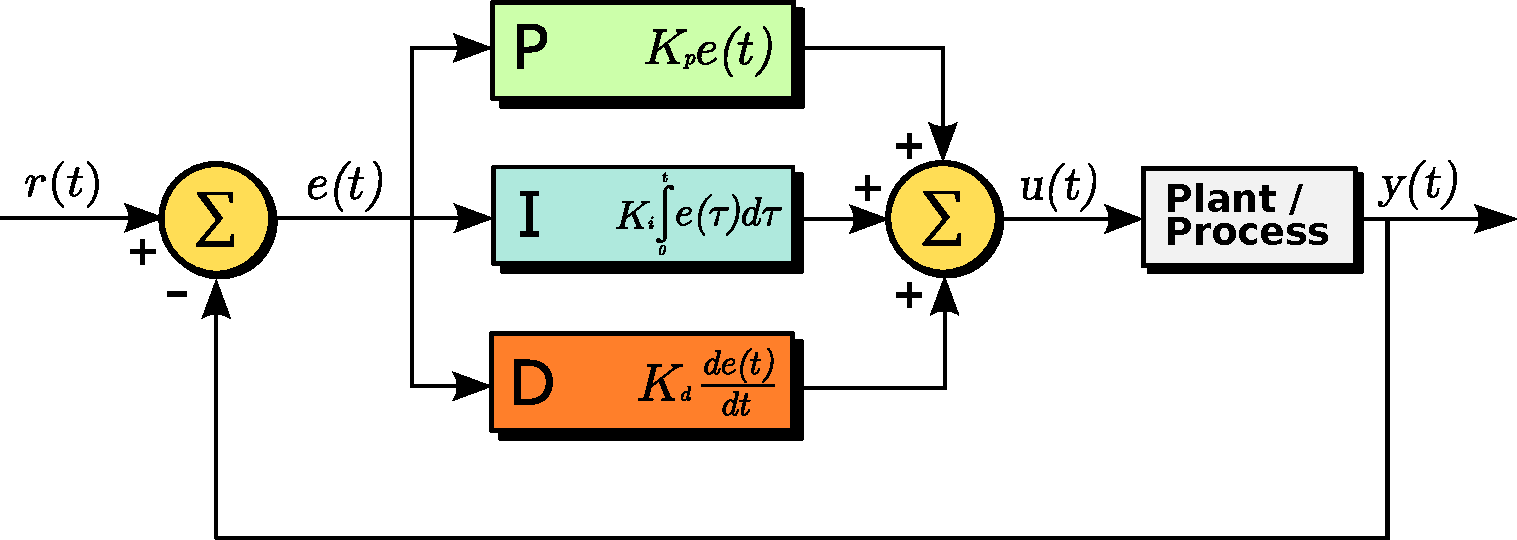
\includegraphics[width=0.85\linewidth]{PID_en.pdf}
        \caption{Sơ đồ khối của bộ điều khiển PID trong vòng phản hồi.}
    \end{figure}
\end{frame}

\begin{frame}{Ứng dụng khác của SOA}
\begin{itemize}
    \item \textbf{Thiết kế bộ lọc số:}
    \begin{itemize}
        \item Tối ưu hệ số bộ lọc IIR.
        \item Đáp tuyến tốt, sai số thấp.
    \end{itemize}

    \item \textbf{Tối ưu hệ thống điện:}
    \begin{itemize}
        \item Phân phối kinh tế, điều phối công suất.
        \item Dùng kết hợp hệ chuyên gia.
    \end{itemize}
    \item \textbf{Căn chỉnh quang học:}
    \begin{itemize}
        \item Dùng CASOA cho căn chỉnh LD và sợi quang.
    \end{itemize}

    \item \textbf{Thiết kế vật liệu:}
    \begin{itemize}
        \item Thiết kế lớp hấp thụ vi sóng nhiều tầng.
    \end{itemize}

    \item \textbf{Học máy – Chọn thuộc tính:}
    \begin{itemize}
        \item ESOA áp dụng trong nhận dạng cảm xúc.
        \item Nâng độ chính xác, giảm thuộc tính dư.
    \end{itemize}
\end{itemize}
\end{frame}











\section*{Ưu và nhược điểm của SOA}


\begin{frame}{Ưu điểm của SOA}
\begin{itemize}
    \item \textbf{Thích nghi thông minh:} Tự động thu hẹp hay mở rộng tìm kiếm theo chất lượng nghiệm.
    \item \textbf{Chất lượng và ổn định:} Nghiệm tốt, kết quả ổn định qua nhiều lần chạy.
    \item \textbf{Trực quan và linh hoạt:} Dễ hiểu nhờ mô phỏng hành vi con người.
    \item \textbf{Không cần đạo hàm:} Áp dụng được cho hàm phi tuyến, không khả vi.
    \item \textbf{Dễ mở rộng:} Hỗ trợ tích hợp chaos, bước nhảy động, lai với thuật toán khác.
\end{itemize}
\end{frame}

% %-----------------------

\begin{frame}{Nhược điểm của SOA}
\begin{itemize}
    \item \textbf{Hội tụ sớm:} Dễ kẹt tại cực trị cục bộ nếu thiếu đa dạng hóa.
    \item \textbf{Chi phí tính toán:} Một vòng lặp phức tạp hơn so với GA, PSO.
    \item \textbf{Khó tinh chỉnh tham số:} Nhiều biến số cần kinh nghiệm để tối ưu.
    \item \textbf{Ít phổ biến:} Cộng đồng nhỏ, thư viện hỗ trợ chưa nhiều.
\end{itemize}
\end{frame}

\begin{frame}[allowframebreaks, noframenumbering]
    \nocite{*}
    \printbibliography
\end{frame}

\begin{frame}
    \begin{block}{}
    \medskip
    \center{\huge \it \textcolor[rgb]{0.37, 0.150, 0.190}{Thanks for listening!}}
    \medskip
    \end{block}	
\end{frame}    
\end{document}
